\documentclass[Main.tex]{subfiles} 
\begin{document}

\subsubsection{Use Case 2: Vis placering af alle busser og stoppesteder p� valgt rute}
Denne Use Case kan startes efter Use Case 1 eller 4 er gennemf�rt. Den startes ved et tryk p� en rute, enten fra hovedsk�rmen eller fra listen af alle busruter. Hovedforl�bet splitter sig alts� op, alt efter hvordan Use Case 2 startes. I OnCreate, hvis det medsendte intent ikke har et favoriserings flag med, s�ttes der ikke en progressbar. Dette g�res, fordi busruten l�ses s� hurtigt ind, at det ikke vil have nogen effekt. Herudover ops�ttes viewet, og der v�lges om der skal l�ses fra SQLite- eller MySQL databasen. Rutenummeret, medsendt i det intent activityet er startet med, s�ttes i informations baren, over kortet. Desuden ops�ttes kortet med det samme, hvis det er en favoriset rute. I OnStart startes servicen, og n�r forbindelsen er oprettet, startes tegningen af ruten baseret p� det valg af database, der blev sat i OnCreate.
\begin{itemize}
	\item \textbf{Favorit rute}
	\begin{itemize}
		\item Samtlige rute IDer hentes fra SQLite databasen. Dette g�res da det er muligt at ruten er kompleks, og bliver gemt som seperate subruter. Herefter bliver hver subrutes stoppesteder og rutepunkter hentet, igen fra SQLite databasen, og disse tegnes p� kortet. Hentningen sker i en seperat tr�d, men rutepunkter og stoppesteder skal s�ttes i main-tr�den, da viewet skal opdateres, og det kun kan g�res fra den tr�d der oprettede viewet. 
	\end{itemize}
	\item \textbf{Ikke favoriset rute}
	\begin{itemize}
		\item Servicen kaldes og den s�rger for at hente busruten og stoppesteder fra MySQL databasen. Ruten kan v�re kompleks, og derfor hentes samtlige ruter og stoppesteder, med det valgte rutenummer. Til hvert stoppested og busrute er der oprettet en speciel designet model klasse, som implementerer parcelable. Denne funktionalitet beskrives i \textit{8.2.1: Komponent 1: Mobil applikation}. Servicen henter det hele i en seperat tr�d. \\
		Servicen s�tter hentede busruter og stoppesteder i en message, og sender den til den medsendte  MessageHandler. I BusMapActivity h�ndteres denne besked i main-tr�den. Progressbaren f�rdigg�res, kortet ops�ttes, og hentede ruter og stoppesteder hentes og tegnes.
	\end{itemize}
\end{itemize}
Ruten best�r kun af de punkter, som ikke er stoppesteder. Stoppestederne kan ligge forskudt for ruten, hvilket ville g�re, at ruten ikke vil f�lge vejene. Ruten bliver indtegnet som en r�d polyline, og stoppestederne bliver indtegnet som et punkt med custom markers. \\

\noindent
Samtidig med ruten hentes og tegnes, startes processen, hvor positionen for busserne hentes. Dette g�res ved et kald til servicen, hvor en messagehandler sendes med. Hentningen sker i seperat tr�d, og k�rer s� l�nge servicen er bundet til viewet. Samtlige hentede positioner sendes tilbage over den medsendte messagehandler, og markerne for bussernes fjernes, hvis de i forvejen er sat, og s�ttes igen med deres nye position. N�r viewet lukkes, unbindes servicen og positionen for busserne holdes ikke l�ngere opdateret. P� figur \ref{fig:UC2SSD}, kan et simpelt sekvensdiagram ses, for processen omhandlende tegning af favorit rute, stoppesteder og bus positioner. Samme sekvensdiagram kan bruges for tegning af en ikke favoriseret rute med stoppested, hvor aktiviteten starter fra BusListMenuActivity, og TrackABusProvider tilg�s i stedet for ContentProviderAcces, for at hente ruten. 

\begin{figure}[H]
	\centering
	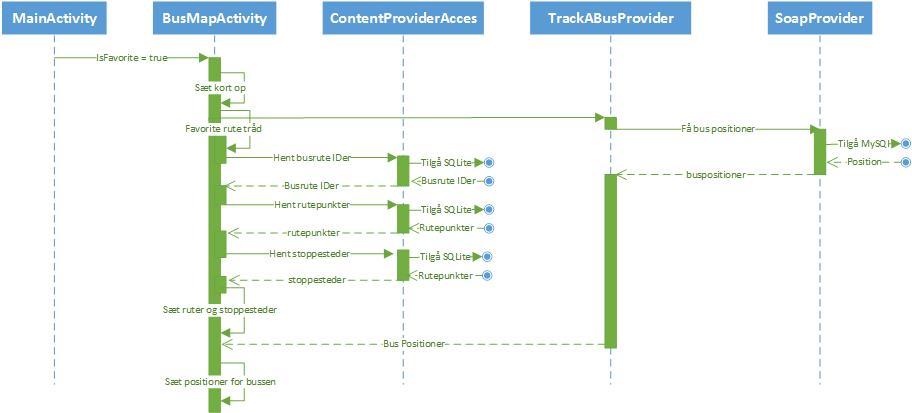
\includegraphics[scale=0.65]{Diagrammer/Sekvensdiagrammer/UC2SSD}
	\caption{Sekvensdiagram for tegning af en favoriseret rute, og hentning af bus positioner}
	\label{fig:UC2SSD}
\end{figure}



\end{document}